\documentclass[tikz,border=8pt]{standalone}
\usepackage{amsmath,amssymb}
\usepackage{fontspec}
\setmainfont{Times New Roman}
\usetikzlibrary{arrows.meta,positioning,calc}

\begin{document}
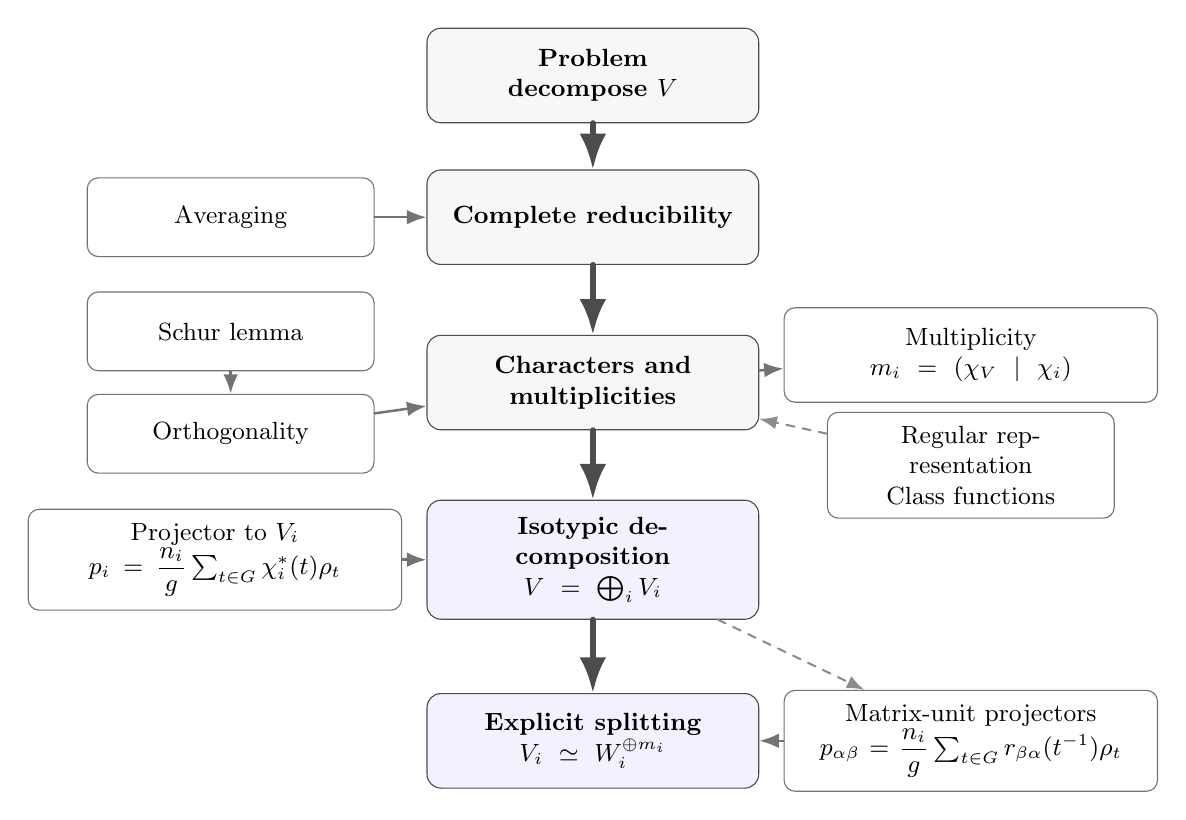
\begin{tikzpicture}[
    >=Latex,
    line cap=round,
    line join=round,
    main/.style={->,line width=2.2pt,black!70},
    link/.style={->,line width=0.9pt,black!55},
    hint/.style={->,line width=0.75pt,dashed,black!45},
    core/.style={
        draw=black!70,
        rounded corners=5pt,
        fill=black!3,
        inner xsep=8pt,
        inner ysep=6pt,
        align=center,
        font=\small\bfseries,
        text width=3.65cm,
        minimum height=12mm
    },
    side/.style={
        draw=black!55,
        rounded corners=4pt,
        fill=white,
        inner xsep=7pt,
        inner ysep=5pt,
        align=center,
        font=\small,
        text width=3.15cm,
        minimum height=10mm
    },
    formula/.style={
        draw=black!55,
        rounded corners=4pt,
        fill=white,
        inner xsep=7pt,
        inner ysep=5pt,
        align=center,
        font=\small,
        text width=4.25cm,
        minimum height=12mm
    },
    result/.style={
        draw=black!70,
        rounded corners=5pt,
        fill=blue!5,
        inner xsep=8pt,
        inner ysep=6pt,
        align=center,
        font=\small\bfseries,
        text width=3.65cm,
        minimum height=12mm
    }
]

\node[core] (problem) at (0,5.8) {Problem\\decompose $V$};
\node[core] (exist) at (0,4.0) {Complete reducibility};
\node[core] (count) at (0,1.9) {Characters and multiplicities};
\node[result] (iso) at (0,-0.35) {Isotypic decomposition\\$V=\bigoplus_i V_i$};
\node[result] (explicit) at (0,-2.65) {Explicit splitting\\$V_i\simeq W_i^{\oplus m_i}$};

\draw[main] (problem) -- (exist);
\draw[main] (exist) -- (count);
\draw[main] (count) -- (iso);
\draw[main] (iso) -- (explicit);

% Existence.
\node[side] (avg) at (-4.6,4.0) {Averaging};
\draw[link] (avg) -- (exist);

% Counting.
\node[side] (schur) at (-4.6,2.55) {Schur lemma};
\node[side] (orth) at (-4.6,1.25) {Orthogonality};
\node[formula] (mult) at (4.8,2.25) {Multiplicity\\$m_i=(\chi_V\mid\chi_i)$};
\node[side] (global) at (4.8,0.85) {Regular representation\\Class functions};

\draw[link] (schur) -- (orth);
\draw[link] (orth) -- (count);
\draw[link] (count) -- (mult);
\draw[hint] (global) -- (count);

% Construction.
\node[formula] (pi) at (-4.8,-0.35) {Projector to $V_i$\\$p_i=\dfrac{n_i}{g}\sum_{t\in G}\chi_i^*(t)\rho_t$};
\node[formula] (pab) at (4.8,-2.65) {Matrix-unit projectors\\$p_{\alpha\beta}=\dfrac{n_i}{g}\sum_{t\in G}r_{\beta\alpha}(t^{-1})\rho_t$};

\draw[link] (pi) -- (iso);
\draw[link] (pab) -- (explicit);
\draw[hint] (iso) -- (pab);

\end{tikzpicture}
\end{document}
